\documentclass[11pt,psfig]{article}
\usepackage{epsfig}
\usepackage{times}
\usepackage{amssymb}
\usepackage{float}

\newcount\refno\refno=1
\def\ref{\the\refno \global\advance\refno by 1}
\def\ux{\underline{x}}
\def\uw{\underline{w}}
\def\bw{\underline{w}}
\def\ut{\underline{\theta}}
\def\umu{\underline{\mu}} 
\def\bmu{\underline{\mu}} 
\def\be{p_e^*}
\newcount\eqnumber\eqnumber=1
\def\eq{\the \eqnumber \global\advance\eqnumber by 1}
\def\eqs{\eq}
\def\eqn{\eqno(\eq)}

 \pagestyle{empty}
\def\baselinestretch{1.1}
\topmargin1in \headsep0.3in
\topmargin0in \oddsidemargin0in \textwidth6.5in \textheight8.5in
\begin{document}
\setlength{\parskip}{1.2ex plus0.3ex minus 0.3ex}


\thispagestyle{empty} \pagestyle{myheadings} \markright{Homework
1: CS 273, Machine Learning: Winter 2015}



\title{CS 273 Homework 1}
\author{Zachary DeStefano, 15247592}
\date{Due Date: Wednesday, January 14, 2015}

\maketitle

\vfill\eject

%\begin{figure}[H]
%\centering
%\includegraphics[height=4in]{prob1plot.jpg}
%\caption{Probability of Class Labels with decision boundaries marked}
%\end{figure}

\section*{Problem 1}

\subsection*{Problem 1, Part a}

The number of features is 4\\
The number of observations is 148\\

\subsection*{Problem 1, Part b}

\begin{figure}[H]
\centering
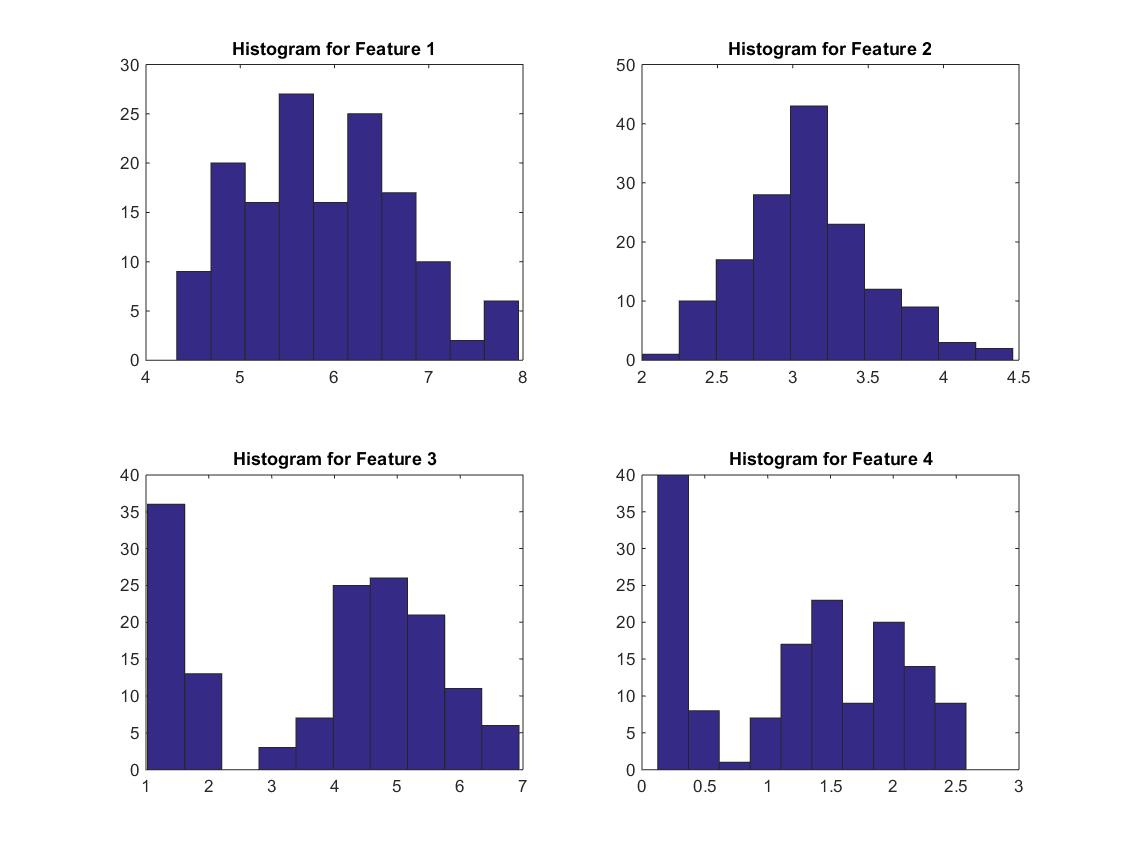
\includegraphics[width=\columnwidth]{prob1bHistograms.jpg}
\caption{Histograms for each feature}
\end{figure}


\end{document}








